% !TeX root = ../main.tex
% Add the above to each chapter to make compiling the PDF easier in some editors.

\chapter{Introduction}\label{chapter:introduction}

\begin{figure}[htpb]
  \centering
  \begin{subfigure}[t]{0.95\textwidth}
    \centering
    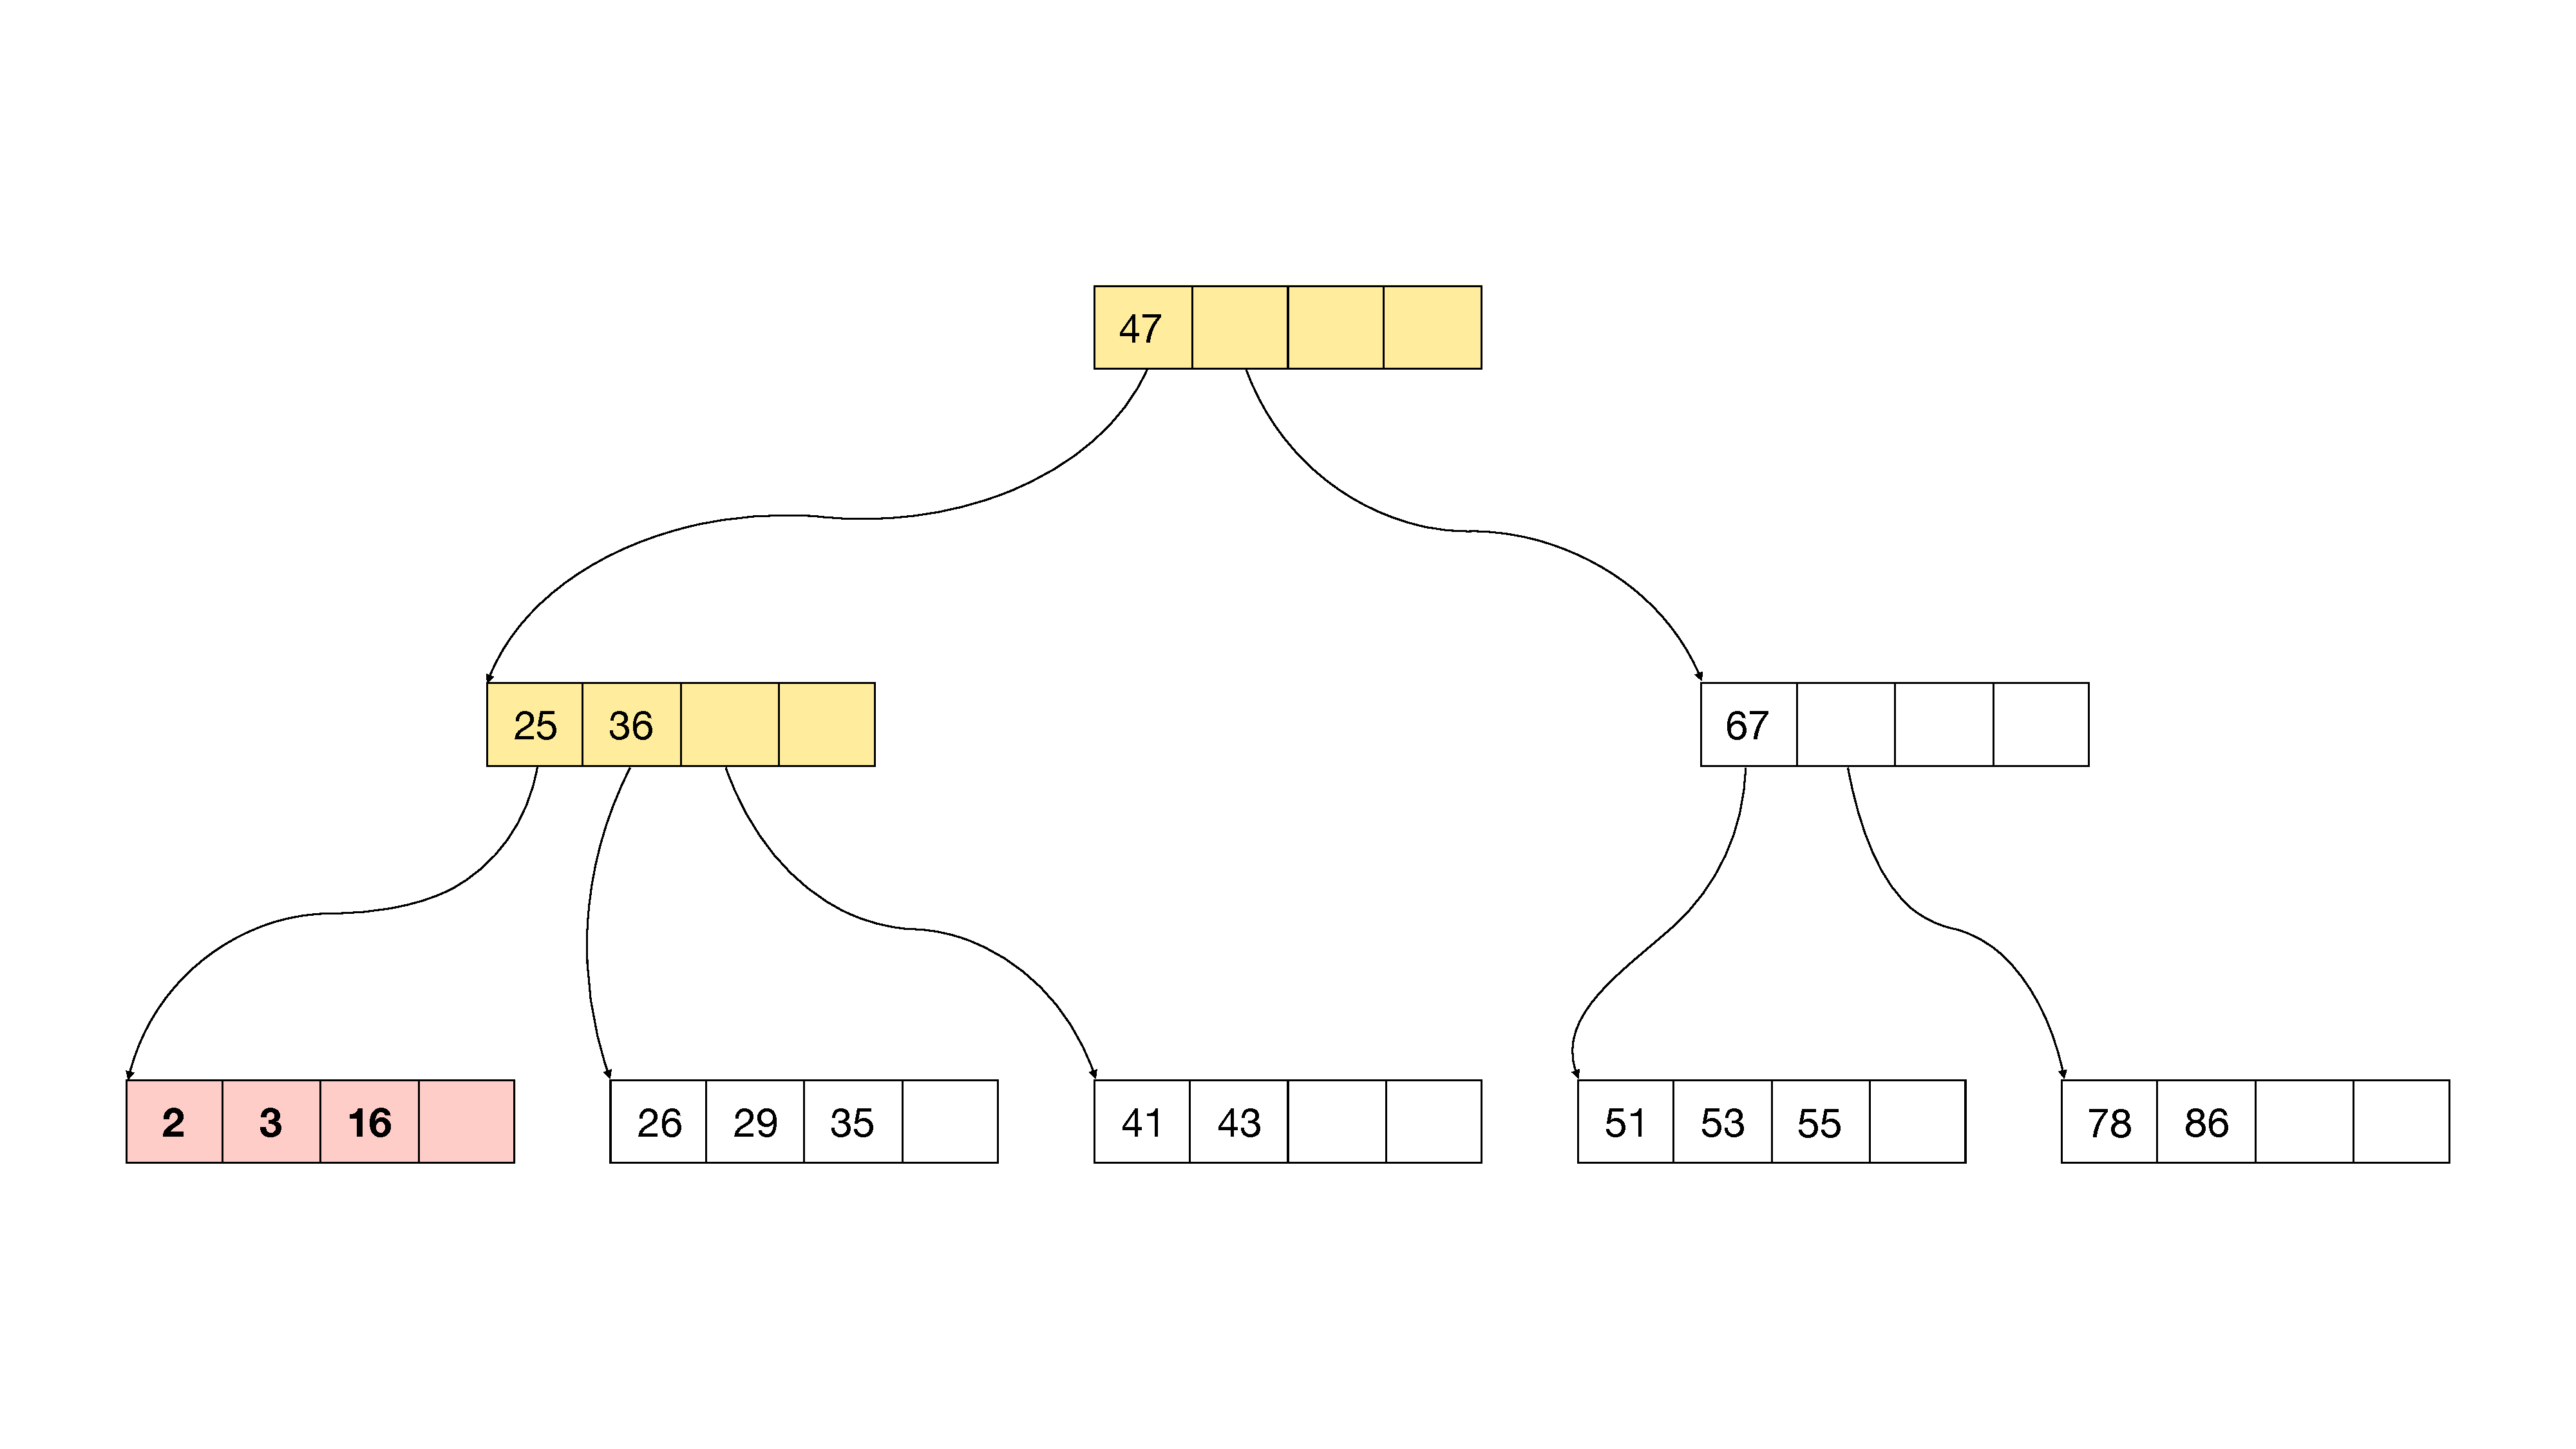
\includegraphics[width=\textwidth]{figures/sequential_access.pdf}
    \caption{Sequential Access Pattern: Updating keys \{2, 3, 16\}.}
    \label{fig:second-pdf}
  \end{subfigure}
  \hfill
  \begin{subfigure}[t]{0.95\textwidth}
    \centering
    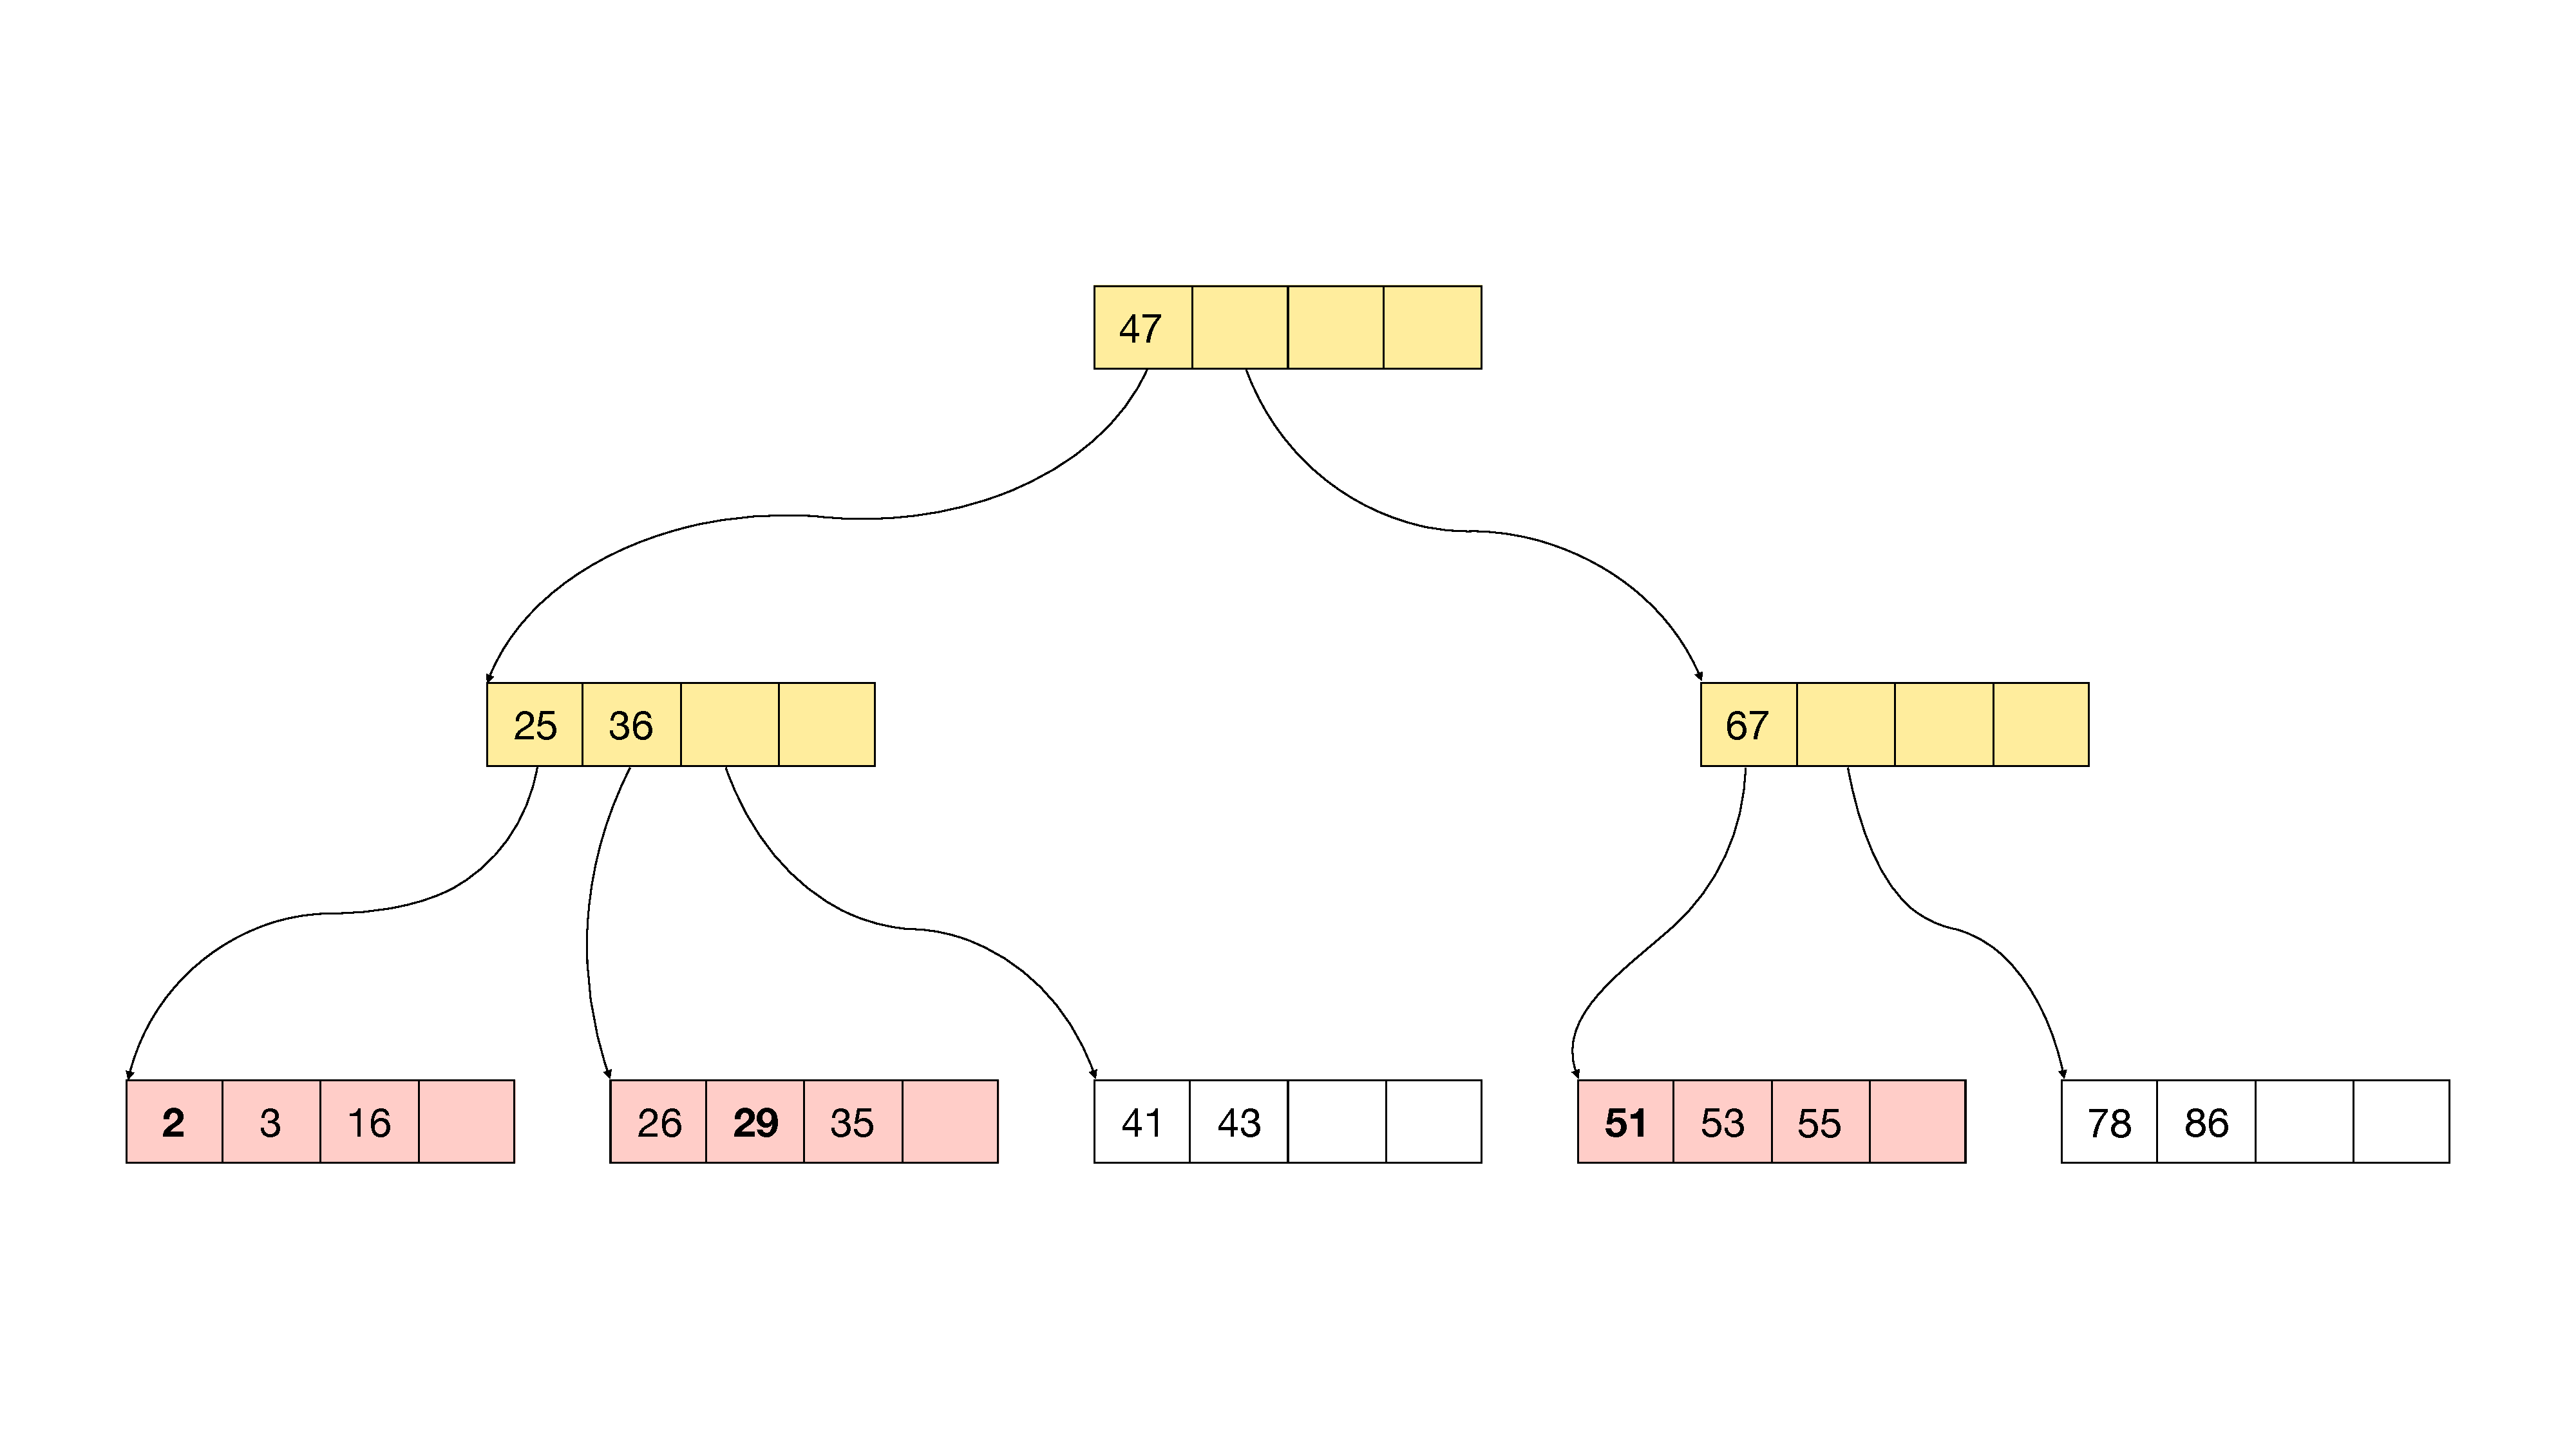
\includegraphics[width=\textwidth]{figures/random_access.pdf}
    \caption{Random Access Pattern: Updating keys \{29, 51, 2\}.}
    \label{fig:first-pdf}
  \end{subfigure}
  \caption{Comparison of access patterns in a B-Tree. Written pages are highlighted in red. Read pages are highlighted in yellow.}
  \label{fig:access-pattern-comparison}
\end{figure}

Efficiently managing large data sets is a core requirement for database systems. 
% Not only have \ac{SSD} become drastically cheaper, they also achieve excellent throughput, making them an attactive, cost-effective storage medium \cite{haas2023modern}.
% Yet, external storage accesses remain magnitudes slower than main memory accesses.
% The largest overhead in beyond memory systems lies in \ac{IO} operations on external storage. 
Therefore, minimizing \ac{IO} operations remains the fundamental premise for designing modern, high-performance \ac{DBMS}.
Primarily, this is done by caching frequently accessed pages in \ac{DRAM} using a buffer manager \cite{leis2018leanstore}.
All data in the system is stored in pages, which the buffer manager can cache and uniformly serve to all components in the system.
This modular design allows a separation of concerns between the buffer manager and its users, such as indexes and data structures.
However, this also means that the buffer manager is agnostic of its user's access patterns.
While the buffer manager minimizes the number of \ac{IO} operations to the best of its knowledge, every component in the systems must design its access patterns to be as efficient as possible. 

A prominent example of such a component is the B-Tree \cite{bayer1970organization}.
B-Trees are the dominant data structure for indexing large datasets in disk-based \ac{DBMS} due to their excellent lookup performance, support for range queries, and simplicity.
However, random writes, a particularly common pattern for secondary indexes, lead to inefficient access patterns that a buffer manager cannot hide for out-of-memory workloads.

B-Trees organize their nodes as pages. Due to their sorted order, accessing random keys leads to random accesses of different pages that need to be loaded into the buffer.
At eviction time, each modified page requires a full rewrite to storage, even if only a small portion of the page changed.
\autoref{fig:access-pattern-comparison} illustrates this effect by comparing a sequential and a random update pattern in a B-Tree.
We consider three updates to the tree.
In the sequential update, only three pages are read and one of them is written to.
In the random update, six pages are read and three of them are written to.
Merely changing the access pattern from sequential to random leads to a threefold increase in the amount of data written to storage.
If we assume that each page is 4 KB, the sequential update requires one storage write of 4 KB.
The random update requires three storage writes of 12 KB in total.
Random writes introduce \emph{write amplification}, a phenomenon where the amount of data written to storage is significantly larger than the amount of data that logically changed.

Write amplification inflates \ac{IO} operations, wastes bandwidth, and ultimately increases latency in bandwidth-bound scenarios.
For example in cloud environments, where storage can be remote, an unnecessary network round-trip directly translates to increased latency and reduced throughput in the system.

Additionally, the \ac{SSD} comes with its own, internal write amplification due to its flash translation layer performing garbage collection \cite{haas2023modern}. 
This leads to a multiplication of unnecessary physical writes, wearing out the device faster.

In summary, to design a truly efficient, high-performance system, we must minimize \ac{IO} operations in all components of the storage stack. 
In this thesis, we focus on closing the efficiency gap in B-Trees by reducing write amplification.

\section{Problem Statement}
% Include metrics for write amplification. Why B-Trees suffer from it. State the gap.
While B-Trees are the backbone of indexing in modern storage engines, their in-place updates introduce significant write amplification, leading to performance degradation and reduced device lifespan. 

\ac{LSMT} address write costs by always writing sequentially, but they introduce high read amplification and complex tuning requirements, making them unsuitable for general-purpose database systems.

B$\epsilon$-Trees buffer and batch updates starting from the root and propagating them down the tree to reduce write amplification. 
Firstly, this introduce two searches per node, one for the next pivot and one for a buffered update for the looked up key.
Secondly, the reduced space for pivots in each node reduces the fanout of the tree, leading to taller trees and more \ac{IO} operations per lookup.
Most importantly though, it significantly limits concurrency in the data structure, as the hottest nodes are locked for longer periods of time to write the update messages, reducing throughput in the tree.

We identify a research gap for a B-Tree variant that effectively reduces write amplification while preserving the excellent query efficiency and concurrency traits of traditional B-Trees.

% Figure: Show write amplification gap between sequential and random writes. Show difference in latency of inserting x keys, difference in IO operations, difference in written volume.

% Circumvent more robust access patterns using LSM Trees. Sacrifice read performance.
\section{Objectives}
% Explicitly list what your thesis adds to the field.
The primary objective of this thesis is to design, implement and evaluate a B-Tree variant that reduces write amplification while maintaining the high read performance and concurrency of traditional B-Trees.
We focus on the following research questions:
\begin{enumerate}
  \item How can we effectively reduce write amplification in B-Trees?
  \item How can we preserve read performance and concurrency in the presence of write optimizations?
  \item How does the proposed approach compare to existing methods in terms of write amplification, query performance and throughput?
\end{enumerate}

While we reflect on significant hardware trends in this thesis, such as the increasing prevalence of \ac{SSD}, we do not target optimizations for specific hardware features.
Instead, we aim to design a solution that is broadly applicable across different storage media and hardware configurations.

We also do not aim to outperform \ac{LSMT} in write-intensive workloads, as they are fundamentally optimized for such scenarios, trading off lookup performance.

While the page-oriented design is one reason for \ac{IO} amplification in B-Trees in general, we do not aim to redesign the data structure from the ground up.
Instead, we focus on a lightweight extension to the traditional B-Tree that can be integrated into existing systems with minimal changes.

\section{Contributions}
% Summarize the main contributions of your thesis.
This thesis introduces 3B-Tree, a B-Tree variant that incorporates a lightweight buffering layer to minimize write amplification.
The buffering layer batches small write operations, reducing the frequency and volume of writes to external storage.
% Instead of changing the B-Tree structure itself, we introduce a secondary data structure, the Delta Tree, that buffers changes to B-Tree nodes.
When a B-Tree node is evicted from memory, we determine whether it has changed significantly enough to warrant a full write to storage.
If not, we buffer the changes.
% When loading a B-Tree node from storage, we apply any buffered changes from the Delta Tree to reconstruct the most recent state of the node.
Essentially, we minimize \ac{IO} operations to those strictly necessary. 

The novelty of our approach lies in its non-intrusive design: We only perform additional operations when B-Tree nodes are exchanged between memory and external storage.
In contrast to other approaches (see \autoref{chap:related-work}), we neither alter the B-Tree structure or its fundamental operations, nor do we impact concurrency or read performance in the tree.
This makes our approach easy to integrate into existing systems and preserves the desirable properties of traditional B-Trees.

We hereby contribute to the broader effort of minimizing overhead of beyond memory systems and designing efficient, high-performance datbase systems for modern hardware.
